\documentclass[reprint]{revtex4-1}
\usepackage{amsmath,amssymb}
\usepackage{graphicx}
\usepackage{cleveref}

\begin{document}
\title{Measurement of the Muon Lifetime}
\author{Daniel Underwood}
\date{\today}

\newcommand{\result}{2.113 \pm 0.002\:\rm{\mu s}}

\begin{abstract}
% TODO: Abstract
% TODO: Change this to tau instead of lambda
A measurement of cosmic ray muons was made with a simple apparatus consisting of a scintillator and a photomultiplier tube. Using an exponential model with a linear least squares fit, the muon mean lifetime was measured to be $\tau_{\mu} = \result$, a $42\sigma$ difference from the 2014 average given by the Particle Data Group.
\end{abstract}
\maketitle

\section{Introduction}
% TODO: Introduction

The importance of the measurement of the muon lifetime is in part due to its relation to the Fermi coupling constant, $G_F$, a free parameter in the Standard Model that is necessary in order to make predictions from the standard model \citep{Chitwood2007,Barczyk2008}. Currently, the uncertainty on $G_F$ is dominated by the uncertainty of the muon lifetime, which drives interest in improving the measurement of the muon lifetime \cite{Chitwood2007}. In addition, the muon lifetime has connections to the weak interaction and special relativity; the former connection is due to the weak interaction being the mechanism of decay for the muon in the reaction given in \cref{eqn: muon-reaction}, while the latter can be seen by the fact that relativistic muons travel long enough to be measured in a laboratory.
\begin{equation}
\mu^{-} \rightarrow \rm{e}^{-} + \nu_{\mu} + \bar{\nu}_{\rm{e}}
\label{eqn: muon-reaction}
\end{equation}

\section{Methods}

The apparatus used for data collection was that described in \cite{Coan2005}. The apparatus captures muons in a scintillator surrounded by the proprietary NE-213 plastic. The light pulse from the scintillator is then amplified by a photomultiplier tube (PMT) and fed through an amplification and discrimination circuit. The signal then reaches a programmable logic controller (PLC) that is able to relay time differentials of the pulses to a computer. These time differentials make up the data that we process.

The data was analyzed using a least squares fit of the form

\begin{equation}
N(t) = N_0 e^{- \lambda t } + B
\label{eqn: fit-model}
\end{equation}
where $N$ is the number of muons at time $t$, $\lambda$ is the decay constant to which the mean lifetime is connected by the relation $\tau = \lambda^{-1}$, and $B$ is a constant factor that counts for background events. For the collected data, Gaussian uncertainties were used so that the errors were given by $\sigma_i = \sqrt{N_i}$ where $N_i$ was the number of counts in data bin $i$. The corresponding bin weights are given by $w_i = \sigma_{i}^{-1}$. $30$ bins were used for separating the data. Using a greater number of bins resulted in bins with zero counts, causing multiple issues. Result differences depending on the number of bins used were negligible providing enough bins were used to accurately model the shape of the exponential. Errors in the independent variable of the fit model were not considered due to the nature of using linear least squares as a fitting technique.

\section{Results}

The collected data along with the proposed fit of the form mentioned in \cref{eqn: fit-model} is shown in \cref{fig: fitted-data}. The fit resulted in finding $\lambda = 0.473 \pm 0.006\:\rm{ps}^{-1}$ with a $\chi^2 / \nu$ value of $0.941$.

\begin{figure}
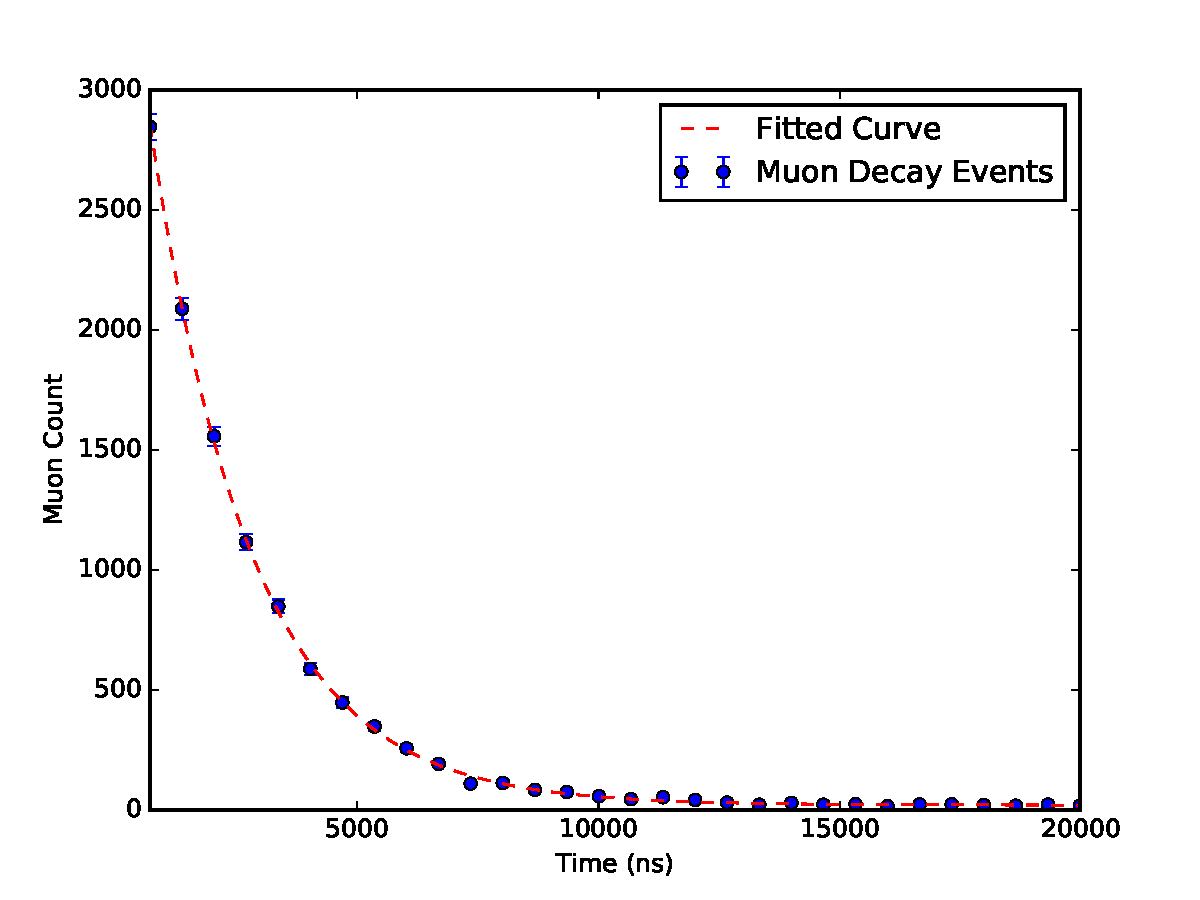
\includegraphics[width=\columnwidth]{../resources/muon-plot.pdf}
\caption{(Color Online) Collected muon lifetimes and fit of the form given in \cref{eqn: fit-model}. Error bars on most points smaller than markers.}
\label{fig: fitted-data}
\end{figure}

Taking $\tau = \lambda^{-1}$ so that the minimum was given by $\tau_{\rm{min}} = \left( \lambda + \sigma_{\lambda} \right)^{-1}$ and the maximum was given by $\tau_{\rm{max}} = \left( \lambda - \sigma_{\lambda} \right)^{-1}$. Using this propagation of errors of $\lambda$, the errors of $\tau$ are given by \cref{eqn: sigma-tau}. Using this result, the muon mean lifetime is found to be $\result$. It should be noted that this method results in asymmetric uncertainties, which in this case were made symmetric due to the uncertainties being the same to one significant figure.

\begin{equation}
\sigma_{\tau}^{\pm} = \left| \lambda^{-1} - \frac{1}{\lambda \pm \sigma_\lambda} \right|
\label{eqn: sigma-tau}
\end{equation}

\section{Discussion}
The most recent $\tau_{\mu}$ average measurement is $2.1969811 \pm 0.0000022\:\rm{\mu s}$ as given by \cite{PDG}. This very large $42\sigma$ discrepancy is expected due to a $\mu^{-}$ being captured and absorbed by a scintillator carbon atom \cite{Chitwood2007}.

Due to this mechanism, the measurement could be improved in future experiments accounting for this process in the model used as the probability of this happening is proportional to the atomic number of atoms in the scintillator \cite{Chitwood2007}. The measurement could be further improved by improvements in the apparatus. One particular area to pay attention to in future experiments is the power source of the apparatus. In this experiment, the apparatus was powered by a source that was not examined for defects in the source or ground.

In future experiments, careful considerations of the differences between $\mu^{+}$ and $\mu^{-}$ should be made. The ratio of their lifetimes is given in \cite{PDG}, which is nearly unity. However, there are differences in the possible sources of error coming from the negative muon and positive muon, such as the capture mechanism mentioned previously only occurring with the negative variety \cite{Coan2005}.

Additional improvements may be made in future experiments by using a longer measurement interval and carefully examining the uncertainties contributed by the timing mechanism and subsequently using a fitting method that takes into account the errors on the independent variable in the fit. In this scenario, the bins can be made the width of the uncertainties in order for the bins to be able to both accurately bin the data and not contribute to further errors.


\bibliography{muon-lifetime}

\end{document}